\section{Prerequisites}

Given the that this paper utilizes mathematical concepts beyond the scope of the IB Mathematics Analysis and Approaches HL curriculum, it is imperative that some notation and important ideas are introduced prior.

\subsection{Notation}
\textbf{Vectors and Matrices.} In this paper, vectors are denoted in 3 main ways based on the context:
\begin{itemize}[leftmargin=!, itemindent=-4ex]
    \item \textbf{$\vec{v}$} -- a letter with an arrow above it denotes a positional vector or translational vector dealing with the transformation of points in space.
    \item \textbf{$\widetilde{v}$} -- a letter with a tilde above it denotes a vector represented in homogenous coordinates. This idea is explained in section \ref{sec:homogenous}.
    \item \textbf{$v$} -- when explicitly stated, a letter without diacritics can also denote a vector if it fails to fall into the categories listed above. 
\end{itemize}
The notation $v^\T$ or $M^\T$ is used to denote the transpose of a vector or a matrix, which is where the rows and columns of the vector or matrix are inverted. 

\subsection{Homogenous Coordinates} \label{sec:homogenous}

While Euclidean space describes 2D and 3D space well, they are not sufficient in describing perspective projections, as it is unable to fully the capture the relationships inherent in projective projections and affine transformations, both of which are core concepts in this paper. 

Homogenous coordinates forms the basis of projective geometry, because it unifies the treatment of common graphical transformations such as rotation and translations \footcite[][1]{bloomenthalHomogeneousCoordinates1994}. 

When
(u,v)


Given the vector $[x, y]^\T \in \mathbb{R}^2$, we can express it in terms of homogenous coordinates: 
\begin{equation}
    \begin{bmatrix}
        x \\ y
    \end{bmatrix}
\end{equation}

\begin{figure}[H]
    \centering
    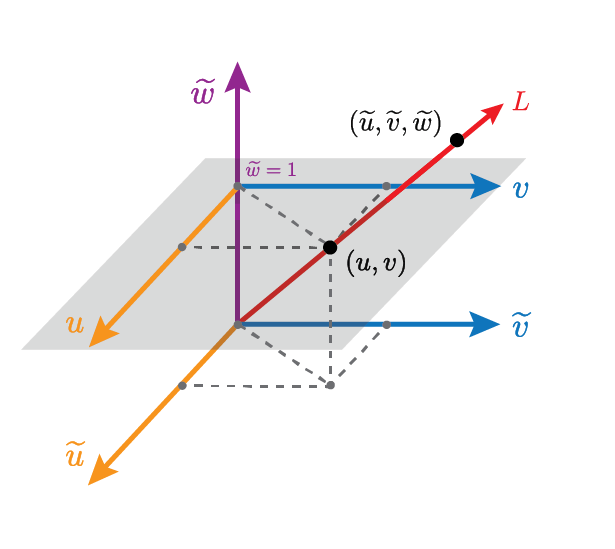
\includegraphics[width=0.6\textwidth]{figures/homogenous}
    \caption{Homogenous coordinate system.}
\end{figure}

In other words, with homogenous coordinates, we interpret our \emph{Euclidean} space as an \emph{affine} space
